\documentclass[11pt,
  a4paper,
  parskip=half, % This is some extra vertical space between paragraphs, the suggestion is 2cm which is really ugly, so we use what koma script gives us
  % you can also set it to full for even more space. But there is a bad tex style decision: parskip also changes the spacing between listitems such as
  % enumerate and itemize. For this purpose we include the enumitem package and set itemsep=.5em, of course you can change this
  BCOR=10mm, % BCOR is binding correction
  english,
  % if you'd rather have a one sided thesis, add `oneside' to the documentclass
  % oneside,
  % ngerman is needed for hyphenation if the thesis contains parts written in German, switch order with english if you write mainly in English.
  % Remember to change order in the babel package (below) as well.
  % Last language is the preferred one.
  % ngerman
  ]{article}
\usepackage{common}

\begin{document}

 
\thispagestyle{empty}
	
	\begin{figure}[H]
	        \minipage[t]{.7\textwidth}
		   	          
\includegraphics[height=4cm]{images/ufreiburg_logo1.png}
			          \label{Logo_ENESJ}
	        \endminipage
	\end{figure}
	
    \begin{center}
    	\vspace{1cm}
    	\huge
	    \textbf{UNIVERSITY OF FREIBURG}
	
    	% \vspace{0.4cm}
    	% \Large
    	% \href{https://www.enesjuriquilla.unam.mx/}{ESCUELA NACIONAL DE ESTUDIOS SUPERIORES}\\
    	% \href{https://www.enesjuriquilla.unam.mx/}{UNIDAD JURIQUILLA}
	
    	\vspace{1cm}
    	\large
    	\today
	
    	\vspace{0.2cm}
    	\large
    	SeminarReport\\
    	April 2022 - Septemper 2022
	
    	\vspace{1.5cm}	
    	\huge
    	\textit{\textbf{Fair and Interpretable Machine Learning}}

	    \vspace{1.5cm}
    	\normalsize	
    	\vspace{0.3cm}
    	\large
    	\yourname
	
        \vspace{0.4cm}
        \normalsize
        TOPIC\\
        \vspace{.3cm}
        \large
        Accumulated Local Effect Plots
	
    	\vspace{0.5cm}
    	\normalsize
    	PROFESSOR\\
    	\vspace{.2cm}
    	\large
        Dr. Janek Thomas
        
    \end{center}
	
\newpage
\pagenumbering{arabic}
\rhead{} % right side of page head
\lhead{2022}

% \twocolumn % text will be splitted into two columns


\tableofcontents
\newpage

\section{Introduction}
An unprecedented boom is currently occurring in machine learning research. There are a lot of examples like \cite{GIBERT2020102526} or \cite{AlphaFold2021} .
More and more algorithms and applications are being discovered in this field of study that show artificial intelligence to be a comparable or even superior alternative to humans.
Examples of this include the analysis of images using computer vision \cite{resNEt}, self-driving vehicles using reinforcement learning \cite{rlDriving}, and the diagnosis of diseases also known as medical AI \cite{aiHealthCare}.
It follows then that the desire for the industry to integrate machine learning pipelines into the application is immense. 

But it so happens that we are asked questions like, "Why is the car braking now?" or "Why does the patient have this disease and not another one?".
Questions that are important to be answered and that we - as humans - can also answer well, but machines struggle with.
Not only might developers be better able to intervene to enhance performance, but they might also be able to make the predictions and judgments of the model understandable and comprehensible in ethically challenging circumstances. 

In this report we will explain why interpretability is a growing area of study and how it benefits model improvement.
Then Accumulative Local Effect (ALE) Plots will be covered next, followed by the presentation of our case study
and a discussion on difficulties encountered during ALE plot implementation.
In order to wrap up this report, we will discuss the limitations of ALE plots. 


\section{Background}
The questions of how to make models interpretable and what different types and levels of interpretability exist will be addressed in more detail in the section that follows. 


\subsection{Interpretability}
It's critical for people to comprehend decisions in the real world \cite{molnar2022}.
This holds true for all kinds of decisions, including ones regarding whether an application was approved, the reason a diagnosis was given at the doctor's office, or whether taking a longer route through the city actually saves time.

We refer to a decision as being interpretable if there is a question about it and a justification is provided.
Or, to paraphrase Miller's statement in \cite{DBLP:journals/corr/Miller17a}, 
"Interpretability is the extent to which a human can understand the cause of a decision."
People trust a decision or person/machine much more if it can be justified, which is one benefit of interpretability.
Similarly, since safety-critical decisions can be contested, interpretability can better ensure the system's security. 
By notifying the developers of machine learning algorithms more quickly when a problem arises, we can also monitor and enhance the performance or fairness of the algorithms.
Whether it be a specific edge case that was overlooked or an inadequate problem formulation.

Along with the expansion of machine learning and the variety of tasks, complexity increases not only in the problems but also frequently in the models \cite{Goodfellow-et-al-2016}.
In the past few years, there has been a growing amount of research and publication in the area of the aforementioned interpretability of models in order to keep track of these ever-more complex models and comprehend what is happening \cite{molnar2022}. 

We provide a brief introduction to the problem of describing it with increasingly complex models in the paragraphs that follow.
We attempt to illustrate how and where interpretability can begin in response to that. 


\subsection{Black- and White-Box Models}
First, let's take a closer look at our model.
Models with a straightforward structure, such as decision trees or linear regression, are excellent when trying to understand how the model arrived at a specific prediction.
White-box models are referred to as such.
Sadly, white box models frequently perform poorly when dealing with tasks that have a high level of feature interaction or generalized high complexity. 

We frequently also require a more complex model, such as a random forest or artificial neural networks, for those complex problems.
These models are acknowledged to be a potent technology and open up many applications, such as the classification of images \cite{resNEt} or the prediction of in-vitro drug sensitivity \cite{drugPredictionRandomForest}, where more straightforward white-box models fall short.
In comparison to the more transparent white box models, they are typically more accurate. 
Contrarily, these models are more difficult to understand than white-box models.
Humans are frequently unable to fully comprehend how a particular decision was made or which input features are more or less compelling than another due to their higher level of internal complexity.
We refer to them as "black-box models" because we can't see right through them by default and the inner workings are essentially hidden.


\subsubsection{Intrinsic or Post-Hoc}
Intrinsic and post-hoc are criteria for interpretability to indicate how interpretability is achived by the method we applied.
If your model is intrinsically interpretable then you do not often need any additional methods to interpret the model. 
The interpretability arises from the properties from the model itself. Like a decision making process that is easy to follow
or a not to complex structure that is easy to comprehend.\cite{molnar2022}

Post-hoc interpretability on the other side is based on the application of other methods to achieve interpretability. 
This could have several reasons either you could achieve a certain level of comparability between different kinds of models,
also between white and black box models, or there is no other way to interpret your model than to apply post-hoc methods. \cite{molnar2022}


\subsubsection{Scope of Interpretability}
You can interpret a model and it's prediction on different levels of detail. 

\begin{itemize}
    \item \textbf{Global, Holistic}: Here you are trying to understand the complete model and how it makes predictions at once. 
    You are able to do so base on the knowledge of all feature distributions and internal parameters. This is the best option when it comes 
    to interpretability but also the hardest one to achieve. \cite{molnar2022}
    \item \textbf{Global, Molecular Level}: Usually humans are not capable of keeping more than 50 parameters or distributions in their 
    short term memory and simultaneously understanding how a model comes up with new predictions. 
    For more complex models however we would dig a bit deeper to a level where we need to understand the basic algebraic calculations. 
    Sadly though single weights in linear models or splits in trees are coupled with many others especially with correlated variables, which makes it even harder to understand for a human. \cite{molnar2022}
    \item \textbf{Local for Single Prediction}: Lets have a more detailed view on one single data instances. Here we want to know how the model
    came up with the single prediction corresponding to a particular data point. But you can also expand this by varying your data point a
    little bit in order to get the local effect. For example different blood pressures have different effects on the risk for a heart attack.\cite{molnar2022}
    \item \textbf{Local for Multiple Predictions}: This is a sort of gray area between local and global methods. You could either take the group as
    the whole dataset and apply global methods or you iterate through the group and apply the local methods for single predictions and analyze those results. \cite{molnar2022}
\end{itemize}


\section{Local Model-Agnostic Interpretability Methods}
% Tradeoff flexability and interpretability Riberto
% To address the problem of black box models scientists are working on different kinds of methods to have a glimpse at the inner workings. % how we can access internal knowledge 
% \subsection{Model Specific and Model Agnostic Methods}

To interpret a model there are different ways to do so. You could choose to only use a model types which are out of the box interpretable (so called white box models). For example a decision tree where you are able to understand every single prediction the tree made by following the path from root to leaf.
This approach often lacks in terms of performance. Performance of model types like decision trees, attention based networks or sparse linear models are often falling behind the performance of so called black box models like:
random forests or a neural networks with millions of parameters. These models are so vastly complicated in their way to produce a prediction that humans are not able to comprehend them this way. 
That leaves us with the problem that on one hand we want to have an interpretable model but on the other hand we also want to have the optimal performance for the specific task. \cite{molnar2022}
One approach to solve this problem is to use distinct post-hoc methods which provide an insight into the decision making process. Existing methods are divided into two classes. Model specific methods which are 
designed specifically to interpret only one model type \cite{molnar2022}. Known examples for this family are the linear weights of a regression or the split points in a tree \cite{molnar2022}. Even if model specific methods work well for certain methods they 
also bring the disadvantage of not being able to be applied on other model types that they were not designed for. The other family is model agnostic methods which separate the explanation from the model itself. As a result of that they come with a bunch of advantages:
\begin{itemize} 
    \item Model flexibility: for model agnostic methods it does not matter if they are applied on a artificial neural network or a random forest. \cite{modelAgnostic}
    \item Explanation flexibility: with model agnostic methods you're not bound to only one form of explanation. For example you could provide a linear formula or have a graphical display. \cite{modelAgnostic}
    \item Representation flexibility: it doesn't really matter how your features are transformed to be suitable for the model, like one hot encoding for categorical features. You could just use the decoded feature 
    formulation without changing the interpretation provided by the methods output. \cite{modelAgnostic}
\end{itemize}
All these advantages make it very tempting to use model agnostic methods.
But being able to apply these methods on many different types of models comes with the downside that incorporating more powerful forms of feedback
- while remaining model agnostic - is difficult\cite{molnar2022}. 


% \begin{itemize}
%     \item separating explanation from the model is being model agnostic
%     \item advatage over model specific -> flexebility, independent from underying machine learning model \\
%     You do not have to develop a differernt framewirk ofr each model type. This laso allows you to compare many models usiong the same metrics This consistency is essential when you want to compare model performace.
%     
%     Riberto 2016
%     
%     \item what are model specifc methods? not really compareable between different models types
%     \item alternatives to model agnostic:
%     - use only interpretable models: disadvantage is the lack of performance compared to black box models (e.g. decision trees, additve models atttention based networks or sparse linear models)
%     Blackbox models: random forest, arbitrary NN 
%     - use model specific task 
%     \item desirable model agnostic aspects
%     - model flexability: egal random forrest oder NN
%     - explanation flexability: linear formula or graphical
%     - representation flexability: able to look at categorical features without one hot encoding
%     
%     - challenge incorporating more powrfull forms of feedback while remaining model agnostic
% \end{itemize}


\section{Accumulated Local Effect}
In the following section we introduce the Accumulated-Local-Effect (ALE), develop an intuition on how they work and have a short look on the definition and estimation.

\subsection{Motivation}
Prior to the introduction of ALE in 2001, partial dependence (PD) plots were state of the art methods to determine the influence of specific feature variables on a prediction \cite{friedman2001greedy}. Unfortunately, PD plots work under the assumption that there are no or very minimal correlations between individual predictor variables. 
This can be seen well in the definition of PD plots.
\begin{equation}
    \hat{f}_{S, PD}(x_S) = \int p_C(X_C) \hat{f}(x_S, X_C) d x_C
\end{equation}
This value returns the value prediction of the model at location $x_S$ averaged over all distributions of the features from $X_C$.
For example $X_C$ is a one-element set with the feature $x_C$, this can be thought of as the projection of all data points 
on the axis $x_C$ onto the value $x_S$. As shown in \figref{fig:PD_M} (a). In the next step we pass the projected data points to the model $f$ 
before we take the predictions from $f$ as a weighted sum with respect to the distribution of the data points on $x_C$. \cite{friedman2001greedy}

\begin{figure}
    \centering
    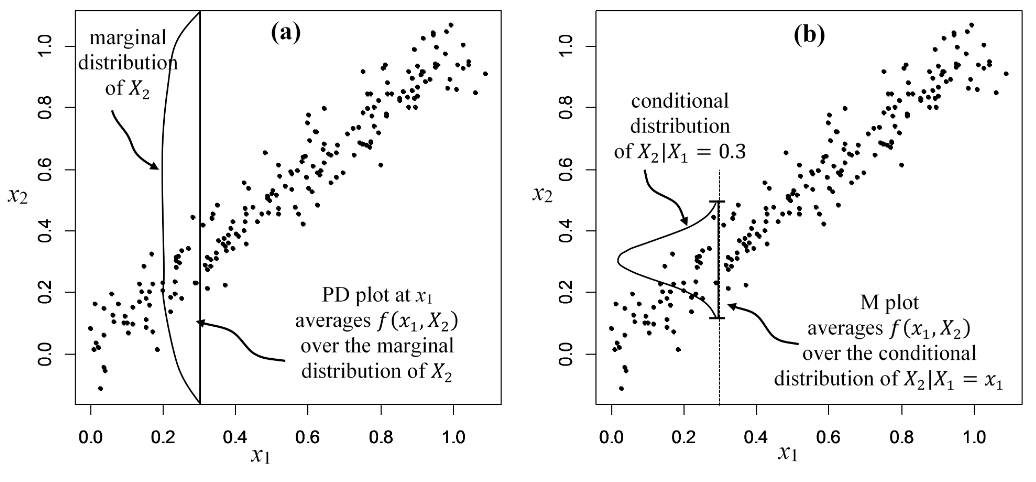
\includegraphics[width=0.7\linewidth]{images/PD_and_M.png}
    \caption{How the the data points are projected on the axis of the predictor variable wen want to look at}
    \label{fig:PD_M}
\end{figure}

Now back to the problem of correlated features. When two or more features correlate, the projection of the 
data points can lead to unrealistic data instances. As an example from the real world we can take the correlation 
between daily temperature and day of the year of a place in southern Germany. If we now project all days of the year
to a temperature of 28°C we get days in August with 28°C as well as days in January with 28°C. This synthetic data can 
lead to a corrupted effect.

This still leaves us with the question on how we solve the problem of correlated predictor variables. 
An approach to solve this problem was the idea tried with Marginal-Plots (M-Plots). In M-Plots we are not extrapolating 
every single data point on our axis. We are only taking data points within a small margin around the actual $x_S$ and extrapolate them shown in \figref{fig:PD_M} (b) \cite{ALE-paper}.
\begin{equation}
    \hat{f}_{S, M}(x_S) = \int p_{C|S}(x_C | x_S) \hat{f}(x_S, X_C) d x_C
\end{equation}
This removes unrealistic data instances, like in the example above, but opens up a new kind of problem if the predictor variables are correlated. If we are using M-Plots we are regressing our prediction on the predictor variable while ignoring every other correlated feature. As a consequence $f_M$ will return a biased effect due to the dependency of our prediction on more than just one predictor variable. This is described as the omitted variable bias phenomenon in regression \cite{ALE-paper}. 

An approach to solve this problem is given by the ALE. 


\subsection{Methology} \label{section:methology}
The Accumulated Local Effect is introduced as an solution to the previous problems of unrealistic data points and the omitted variable bias phenomenon \cite{ALE-paper}. 
First we want to start to describe the method using the estimation of the Accumulated Local Effect because it is a bit more digestable than the definition. 

Afterwards we divided our data into buckets as shown as in \figref{fig:1dbuckets}. The final bucket shape depends on how many buckets we want to have and how many 
elements one buckets should contain. You can find a more detailed description on how to create those buckets in \secref{section:Implementation}. 
After this we iterate over each bucket and calculate the local effect. To calculate the local effect for a bucket with index $k$ we have to do four things for each bucket $N_j(k)$: 
\begin{enumerate}
    \item shifting every predictor variable $z$ of each data instance to the \textbf{upper} border of the bucket without changing any other value $x_{\backslash j}^{(i)}$ and get their prediction from the model  $\overset{\sim}{f}(z_{k, j}, x_{\backslash j}^{(i)}) $
    \item shifting every predictor variable $z$ of each data instance to the \textbf{lower} border of the bucket without changing any other value $x_{\backslash j}^{(i)}$ and get their prediction from the model  $\overset{\sim}{f}(z_{k-1, j}, x_{\backslash j}^{(i)})$
    \item calculating their difference:  $\overset{\sim}{f}(z_{k, j}, x_{\backslash j}^{(i)}) - \overset{\sim}{f}(z_{k-1, j}, x_{\backslash j}^{(i)})$ 
    \item calculating the mean: $\frac{1}{N_j(k)} \sum_{i:x_j^{(i)} \in N_j(k)}\left[ \overset{\sim}{f}(z_{k, j}, x_{\backslash j}^{(i)}) - \overset{\sim}{f}(z_{k-1, j}, x_{\backslash j}^{(i)})\right]$
\end{enumerate}
After we have done this we get something like the local effects shown in the left graph of \figref{fig:local-effects}. To complete the algorithm, we only have to accumulate all local effects. All this adds up into our estimation formula: \cite{molnar2022}
\begin{equation} \label{eqn:ALE-Estimation}
    \hat{\overset{\sim}{f}}_{j, ALE}(x) = \sum_{k = 1}^{k_j(x)} \frac{1}{N_j(k)} \sum_{i:x_j^{(i)} \in N_j(k)}\left[ \overset{\sim}{f}(z_{k, j}, x_{\backslash j}^{(i)}) - \overset{\sim}{f}(z_{k-1, j}, x_{\backslash j}^{(i)})\right]
\end{equation}
An exemplary result can be seen on the right hand side of \figref{fig:local-effects}. 

\begin{figure}
    \centering
    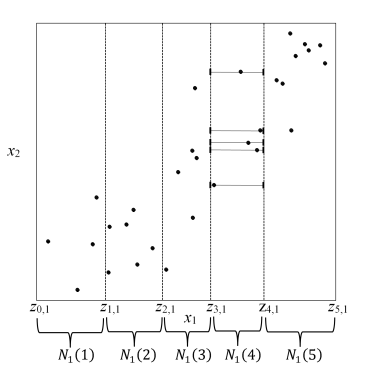
\includegraphics[width=0.3 \linewidth]{images/1DBuckets.png}
    \caption{Displayed is a correlated data distribution over $x_1$ and $x_2$ which is partitioned into five buckets $N_1(1)$ to $N_1(5)$. The splitting points are $z_{0,1}$ to $z_{5,1}$}. For bucket number four it is illustrated how the data points are shifted between the bucket limits.
    \label{fig:1dbuckets}
\end{figure}

\begin{figure}
    \centering
    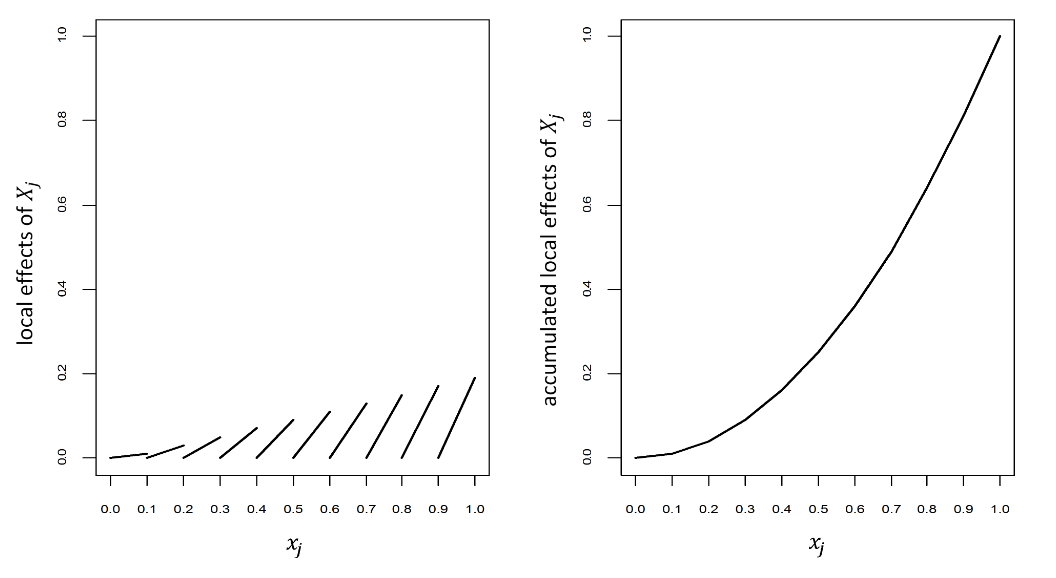
\includegraphics[width=0.7\linewidth]{images/local_effects.png}
    \caption{Ground truth for those two graphs is quadratic effect of feature $x_j$. On the left hand side are the local effect as linear function inside the bucket. The slope is the actual local effect divided by the bucket width. You can see here that the tips of the linear function show a also a linear function, the derivative of the ALE. On the right hand side you can see the accumulated sum of the local effects from the left plot.}
    \label{fig:local-effects}
\end{figure}

Now we are able to see constant, linear, quadratic or any other polynomial effect in the plots. But before we can now jump into an interpretation on the value level we first have to center the plot. This means subtracting the average prediction from every ALE, as stated in \eqref{eqn: cenetered-ALE-estimate}. \cite{molnar2022}
\begin{equation} \label{eqn: cenetered-ALE-estimate}
    \overset{\sim}{f}_{j, ALE}(x) = \hat{\overset{\sim}{f}}_{j, ALE}(x) - \frac{1}{n} \sum_{i=1}^n \hat{\overset{\sim}{f}}_{j, ALE}(x_j^{(i)})
\end{equation}
\eqref{eqn: cenetered-ALE-estimate} works under the assumption of uniformly wide buckets. We will elaborate on this in \secref{section:Implementation}. 
Now we are able to allow following interpretation. For example, from \secref{section:Application} an ALE estimate of $0.2$ at $x_\text{ejection\textunderscore fraction}=22$ from \figref{fig:ALE-1/ejection-fraction} means that when we have an ejection fraction of 20, then the prediction of a death event is higher by 0.2 compared to the average prediction.


\subsection{Definition}
Now lets turn our attention onto the theoretical part of ALE plots. Starting with the formula with which a first order effect - where we saw it's estimation previously - is calculated. \cite{molnar2022}
\begin{equation}
    \hat{f}_{S, ALE}(x_S) = \int_{z_{0, S}}^{x_S} \mathbb{E}_{X_C \mid  X_S=x_S}\left[\hat{f}^S(X_s, X_x) | X_S = z_S\right] dz_S - \text{constant}
\end{equation}

\subsection{Properties and Comparison to PD- and M-Plots}
Here I would like to go into several different properties of ALE plots.

\textbf{No unrealistic data instances}. \\
While we motivate ALE plots during the first subsection we had a brief look in to partial dependence plots. The big problem with those was the massive amount of extrapolation we have to do. Now we avoid this problem with ALEs by the introduction of buckets and extrapolating only inside a bucket.
So they don't have the assumption of uncorrelated features which is a big advantage over PD-plots. \cite{ALE-paper}

\textbf{Avoiding the Omitted Variable Bias}\\
Due to the pairwise differences of model predictions in a bucket. We also avoiding the omitted variable bias because of the pairwise differences that block any other nuisance variable. \cite{ALE-paper}

\textbf{Extensions} \\
In the paper there are additional methods described how to apply also a second order effect to illustrate how two predictor variables are working together and how we are able to apply ALE on categorical features. \cite{ALE-paper}\cite{molnar2022}


\section{Case Study}
In this section we will present a case study we conducted in order to show some examples of ALE plots. You can find the git repository at \texttt{https://github.com/RobinU434/AccumulatedLocalEffectPlots}.


\subsection{Implementation} \label{section:Implementation}
In the case study I implemented the first order ALE plot for continuous features myself. The signature for this function looks like the following:
\begin{verbatim}
    ale( model,
         X: pd.DataFrame,
         grid_shape: Tuple,
         columns: Tuple,
         show: bool = False,
         std: np.array = np.ones(100), 
         mean: np.array = np.zeros(100)
        )
\end{verbatim}
To apply this function you need a pre-trained model that contains the method predict. Also you need to provide the dataset on which you would like to operate on, the feature name for the tuple \texttt{columns} and the number of bucket embedded in \texttt{grid\textunderscore size}.
The arguments \texttt{std} and \texttt{mean} are more optional. Through those values you are able to provide the original distributional properties of the data in case you are using normalized data.
It is likely that you need this option if you are working with black box models like neural networks \cite{Goodfellow-et-al-2016}.

In the following I would like to have a bit more detailed look into the implementation. 
Based on the previous knowledge of how we can estimate the ALE based on \eqref{eqn:ALE-Estimation}. This step seems to be really straight forward. But during the implementation I encountered several problems with the buckets here referred as: $N$.

First we have to divide our feature space into buckets. How you do this is not perfectly described by the paper \cite{ALE-paper}. 
There are two possibilities to do so. 

The first option is to choose a constant bucket width with respect to the maximum and minimum
of the features you want to have an insight into. This is also implied in the paper by the centralization of the estimated ALE as in \eqref{eqn: cenetered-ALE-estimate}. Here the computation of the mean as in \eqref{eqn: cenetered-ALE-estimate} works if and only if, the 
distribution of the local effects, and so also our buckets, is uniform over the feature space of our predictor variable.

Nevertheless this possibility has the advantage of only being dependent on the local effect and not on the bucket width. 
That leads to a more consistent interpretation over the feature space of your data set.
On the downside in regions with a sparse data distribution it could happen that some buckets are empty,
like in \figref{fig:ALE-1/creatine-phosphokinase} on the right hand side.
This would lead to a huge uncertainty and a division by zero for these empty buckets
($1/N$ in \eqref{eqn:ALE-Estimation} with $N =  0$) which is not describable by the method. 

The second option is to sort the corresponding data points by the feature of interest and select a constant number of 
data points for each bucket. This would eliminate the problem with the empty buckets but opens the problem of inconsistent 
bucket-widths. This ends in the issue that we need another function to center the ALE. In contrast to a constant bucket width this is a bit more complicated and computationally intensive because the assumption of a constant bucket width with respect to the feature space does not hold anymore.
Therefore you now have to use the following mean calculation:
\begin{equation*}
    \overline{f} = \frac{1}{b-a} \int_a^b f(x) dx
\end{equation*}
In the implementation this is done by
\begin{verbatim}
    ale_scores -= np.trapz(ale_scores, quantiles) / (quantiles[-1] - quantiles[0]) 
\end{verbatim}

Because of the less troubling disadvantages we went with the second approach in the implementation, with a constant number of elements in each bucket. 

\subsection{Application} \label{section:Application}
The user study is a binary classification problem on the data set of heart failure, provided by Kaggle (\texttt{https://www.kaggle.com/datasets/andrewmvd/heart-failure-clinical-data}). As the label to predict we will go for \texttt{DEATH\textunderscore EVENT}. For the input features we select: 
age, anaemia, creatinine\textunderscore phosphokinase, diabetes, ejection\textunderscore fraction,	high\textunderscore blood\textunderscore pressure, platelets, serum\textunderscore creatinine, serum\textunderscore sodium,	sex, smoking and time.
As a model we will use a MLPClassifier from sklearn with the following properties:
\begin{itemize}
    \item architecture: 12, 100, 2
    \item activation function: ReLu
    \item learning rate: 1e-4
    \item optimizer: adam
    \item momentum: 0.9
\end{itemize}
With these properties we are able achieve between 73\% and 85\% accuracy.
The results of my ALE applications are displayed in \figref{fig:ALE-1} and \figref{fig:ALE-2}.

Interpretation for \figref{fig:ALE-1}:
\begin{enumerate}[label=(\alph*)]
    \item Displayed in \figref{fig:ALE-1/age} is the patients age. Here we can see a relatively strong effect - in comparison to most of the other features - with something that's seems to be a quadratic relation. 
    \item Displayed in \figref{fig:ALE-1/creatine-phosphokinase} is the creatine phosphokinase level in the blood.
    Creatine is a molecule, that can store and provide energy rapidly and for a short amount of time if needed. CK is an enzyme that facilitates the transfer of a phosphate of creatine to ADP (adenosine-diphosphate) to generate ATP (adenosine-triphosphate), which is the most important energy providing molecule in the cell. In healthy tissue, CK is only found intracellularly, so an elevated level of CK in the blood indicates tissue damage and cell death. Different isoforms of CK can be found in different cell types. An elevated blood level of the CK isoform of the heart shows tissue damage of the heart, as it can for example occur in a heart attack \cite{heinrich2014lofflerpetrides}. 
    If we look at the gray curves we can observe something very interesting. It seems we have a lot of variance between those models in the beginning and a bit more stable behavior right at the back. But if you look closely at the data distribution we can see that there are just a few data points with a value higher than 4000. So for this case we should concentrate more on the left hand side. Here we can see that the blue mean curve is indicating a very slight linear effect.  
    \item Displayed in \figref{fig:ALE-1/ejection-fraction} is the ejection fraction. 
    The ejection fraction is the fraction of blood in the ventricle that is pushed out of the heart with each contraction. Usually, the ejection fraction is around 50\%-65\%. It seems plausible, that a reduced ejection faction might be connected to heart failure \cite{TMV}.
    The interpretation here is a bit more obvious. We have a very stable behavior across the models with a tight envelope around the mean. The effect indicates a linear relation between 78 and 25. After this a stronger linear effect than before, that a death event is more likely with a ejection fraction lower than 20. 
    \item Displayed in \figref{fig:ALE-1/platelets} is the  count of platelets in the blood. 
    The number of platelets in the blood does not seem to have a striking correlation to the occurrence of heart failure. Nevertheless, some evidence points toward the importance of platelet activation for the occurrence of secondary events like strokes and thromboembolies. The condition of heart failure might contribute to the abnormal activation of platelets and the formation of clots \cite{10.1093/eurheartj/ehl305}. 
    In contrast to the ejection fraction there is a more widely distributed set of ALE functions across the models. 
\end{enumerate}
Interpretation for \figref{fig:ALE-2}:
\begin{enumerate}[label=(\alph*)]
    \item Displayed in \figref{fig:ALE-2/serum-creatine} is the creatine level in the blood serum. 
    Creatinine is a waste product of creatine that is eliminated by the kidneys. An elevated serum creatinine level seems to be connected to heart failure. A possible explanation might be, that the abnormal heart function and changes of blood pressure in the venous system can lead to abnormal kidney function, like reduced glomerular filtration. Since creatinine is eliminated in the kidneys, reduced filtration might lead to elevated serum creatinine levels \cite{Srivastava22}.
    Here it is almost the same as for the creatine phosphokinase. We have a lot of data points in the beginning and just a few on the right hand side. therefore I would like to concentrate a bit more on the left hand side which indicates a linear relation up to the value 2. Until 4 we also have a more linear effect but not as strong as before.
    \item Displayed in \figref{fig:ALE-2/serum-sodium} is the sodium level in the blood serum. 
    Higher serum sodium levels seem to correlate with a decreased risk of heart failure. However, an explanation for that is difficult to find as we did not find any data in the literature regarding this topic.
    Here the interpretation also a bit difficult because of more widely distributed ALE functions with respect to the actual effect scale ($\approx 0.2$). But in comparison to the other effects we could say that is more like a two stage linear effect between 125 and 145. 
    \item Displayed in \figref{fig:ALE-2/time} is the follow up time in days that refers to the stated length of time a person's health will be monitored over time after a therapy or intervention. The curve shows something like a decreasing sloped step function. This also makes sense because severe cases with intensive treatment are needed to be watched longer than other cases. This lowers the probability that a heart failure will occur after such a long time of monitoring. 
\end{enumerate}

\begin{figure}[htp!]
    \begin{subfigure}[t]{.49\textwidth}
        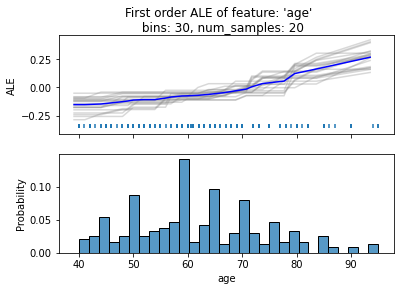
\includegraphics[width=\linewidth]{images/ALE_age.png}
        \caption{}
        \label{fig:ALE-1/age}
    \end{subfigure}
    \hfill
    \begin{subfigure}[t]{.49\textwidth}
        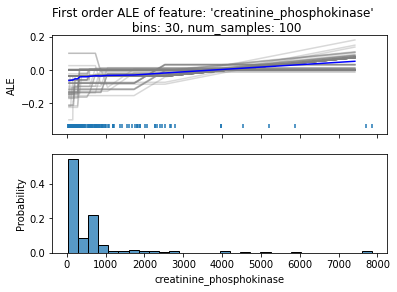
\includegraphics[width=\linewidth]{images/ALE_creatine_phosphokinase.png}
        \caption{}
        \label{fig:ALE-1/creatine-phosphokinase}
    \end{subfigure} \\
        \begin{subfigure}[t]{.49\textwidth}
        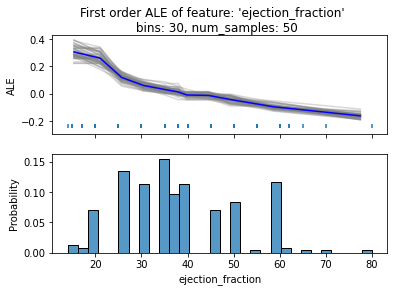
\includegraphics[width=\linewidth]{images/ALE_ejection_fraction.png}
        \caption{}
        \label{fig:ALE-1/ejection-fraction}
    \end{subfigure}
    \hfill
    \begin{subfigure}[t]{.49\textwidth}
        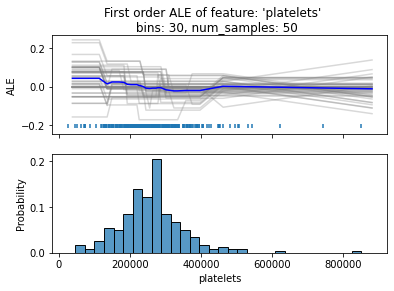
\includegraphics[width=\linewidth]{images/ALE_platelets.png}
        \caption{}
        \label{fig:ALE-1/platelets}
    \end{subfigure}
    \caption{ALE plots for age, creatine phosphokinase, ejection rate and platelets. The upper figure displayes the centered ALE on the y axis and the feature on the shared x axis. The gray lines displaying an ALE of a single model and the solid blue one the aggregated mean. The little ticks on the bottom are representing a single datapoint each. The second plot beneath the actual ALE plot shows the data distribution. }
    \label{fig:ALE-1}
\end{figure}

\begin{figure}[htp!]
    \begin{subfigure}[t]{.49\textwidth}
        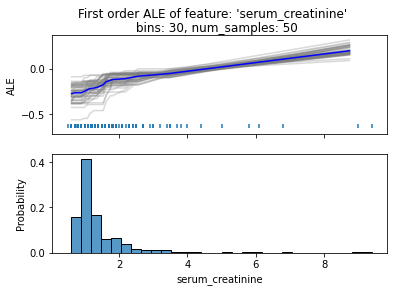
\includegraphics[width=\linewidth]{images/ALE_serum_ceatinine.png}
        \caption{}
        \label{fig:ALE-2/serum-creatine}
    \end{subfigure}
    \hfill
    \begin{subfigure}[t]{.49\textwidth}
        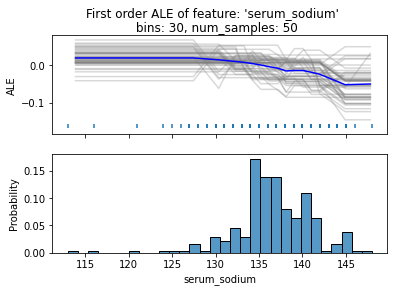
\includegraphics[width=\linewidth]{images/ALE_serum_sodium.png}
        \caption{}
        \label{fig:ALE-2/serum-sodium}
    \end{subfigure} \\
    \begin{center}
        \begin{subfigure}[t]{.49\textwidth}
            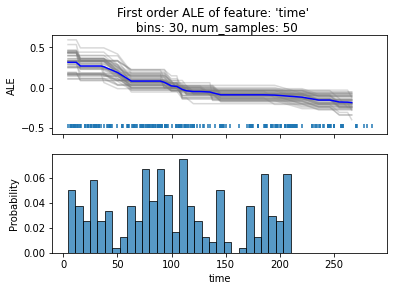
\includegraphics[width=\linewidth]{images/ALE_time.png}
            \caption{}
            \label{fig:ALE-2/time}
        \end{subfigure} \\
    \end{center}
    \caption{ALE plots for serum creatine, serum sodium and follow up time. The upper figure displays the centered ALE on the y axis and the feature on the shared x axis. The gray lines displaying an ALE of a single model and the solid blue one the aggregated mean. The little ticks on the bottom are representing a single data point each. The second plot beneath the actual ALE plot shows the data distribution. }
    \label{fig:ALE-2}
\end{figure}

Last but not least we have the binary features as displayed in \tabref{tab:binary-ALE}. For binary feature we are only able to calculate a single ALE because more than one bucket would lead to unrealistic data points. In general we can observe that the effects are in comparison a lot smaller than we are able to observe in the continuous features.
\begin{table}[htp!]
    \centering
    \begin{tabular}{l l l}
         \textbf{feature} &  \textbf{local effect} & \textbf{std}\\
         \hline \hline
         anaemia & -0.02705718 & 0.01116109 \\
         diabetes & -0.00167364  & 0.00981853 \\
         high blood pressure & -0.01478382 & 0.00738533\\
         sex & -0.05048815 & 0.01158189 \\
         smoking & 0.00585774 & 0.01083566\\  
    \end{tabular}
    \caption{local effect for binary features sampled over 30 sampled models with their standard distribution. The difference is calculated like described in \eqref{eqn:ALE-Estimation} (higher - lower)}
    \label{tab:binary-ALE}
\end{table}


\section{Limitations} \label{section:pot-ext/limit}

Despite all the mentioned advantages of ALE plots there are still several disadvantages. 

First disadvantage is that the interpretation of the effect across buckets is not permitted \cite{molnar2022}. Therefore we are only able to interpret the value of one interval like demonstrated in \secref{section:methology} or interpret the graph as a whole to observe the effect of the feature. 

A second disadvantage is in relation to which method we use to determine the buckets. Not only are there two possible ways to do so but there also remains the problem that the amount of buckets opens up a new hyper parameter that is needed to be tuned. If there are too few buckets we could miss some interesting effects. If there are too many the plots becomes quite messy \cite{molnar2022}. 

Further we want to discuss the second order effect. The second order effect is used to determine the ALE dependency of two predictor variables. If those two variables are correlated we have a lot of cells that are very varying in size, because if we use quantiles as a grid we could end up with very sparse regions. This makes it even harder to interpret constant, linear or any other effect across the grid cells \cite{molnar2022}. Additionally we don't have a practical way to incorporate the aggregation of sampled models. To show how the models local effect is differing across the models we, can't simply have them in the background as in the one dimensional case. We have to use a second plot where we can show some kind of similarity measurement across the models over the two dimensional feature space.  


% A big limitation of ALE plots comes with the second order effect. As we have seen in the first order effect plots in \secref{section:Application}. The underlying model could be a bit shaky and do not converge to the same solution every single time. For the first order effect we were able to visualize this but for the second order effect it is very hard to show this kind of information to the user. Maybe with a second heatmap that shows a metric of similarity between the individual functions.  % 

% In this section I would like to meantion the problem of how to design the buckets and fill respectively with data. As stated before we have on the one hand the approach to use a constant width and on the other and a constant number of elements. Here I would like to propose a way to mitigate the disorted effect a bit. I would like to extra/- interpolate the effects of the % 

% An antidot for this effect could be an additional 
% weighting of the local effects with the individual bucket widths in feature space. This would normalize the local effects but in regions with 
% a low data density the individual bucket width could be to high. This would result in overstepping a ground truth effect and returning a misleading interpreation. \todo{example}% 
% 

% Extension: Take bucket internal extrapolation into account?
% squaring the distance from each datapoint to the middle of the corresponding bucket -> shifted data points are not to different to  
% best: 




% Limitation: \\
% Binary labels could represent someimes a problem because they can indicate a something contraintuitive % 

% But there is a problem with binary features. In Section \ref{section:pot-ext/limit} we will have a bit more detailed look into that. But here I will anticipate a but that is only plausible to compute a single local effect with repsect to the downsides of PD Plots we meantioned befor 
% like creation of unrealistic data points. Therefore I will provide in \tabref{} a short summary of the single local effect from the binary features. You can think of those as the mean increase or decrease of getting a death event with repsect to the corresponding feature. But as I said before
% you are not able to have a look if the feature has a linear, quadratic effect over the feature. % 

% After reviewing both possibilities wew can  conclude that we are not able to overcome data density problem by choosing one or  the other bucket filling technique. % 
% 

% Potential extension:
% I've never encoutered an implementation of a 2D Ale plot only with categorical or mixed with continuous features.
\bibliographystyle{IEEEtranN}
\bibliography{bibliography}

\end{document}